\documentclass[conference]{IEEEtran}
\IEEEoverridecommandlockouts
\usepackage{cite}
\usepackage{amsmath,amssymb,amsfonts}
\usepackage{algorithmic}
\usepackage{graphicx}
\usepackage{textcomp}
\usepackage{xcolor}
\usepackage{ragged2e}
\usepackage{float}
\usepackage{setspace}
\usepackage{hyperref}
\usepackage{url}

\hypersetup{
    colorlinks=true,
    linkcolor=blue,
    citecolor=green,
    filecolor=magenta
    urlcolor=blue,
    pdftitle={Your Document Title},
    pdfauthor={Your Name},
    pdfkeywords={Keyword1, Keyword2, Keyword3},
}


\usepackage[ruled,vlined]{algorithm2e}
\usepackage{amsmath}
\usepackage{amsfonts}

\usepackage{tocbibind} % Đưa mục tài liệu tham khảo vào mục lục
\setcounter{tocdepth}{1} % Mức độ hiển thị trong mục lục

\usepackage{listings}
\lstset{
    basicstyle=\ttfamily,    % Font monospace
    frame=none,              % Không viền
    xleftmargin=1.5em,       % Thụt lề trái
    breaklines=true          % Tự động xuống dòng
}
\usepackage[T5]{fontenc} 
\usepackage[utf8]{inputenc}
\usepackage[vietnamese]{babel}
\usepackage[a4paper, twocolumn, columnsep=22pt, left=0.5in, right=0.5in, top=1in, bottom=1in]{geometry}

\def\BibTeX{{\rm B\kern-.05em{\sc i\kern-.025em b}\kern-.08em
    T\kern-.1667em\lower.7ex\hbox{E}\kern-.125emX}}
\begin{document}
\justifying

\title{Thiết kế và phân tích các thuật toán\\
Tìm kiếm các tập mục hữu ích cao Top-K từ cơ sở dữ liệu không chắc chắn\\
\small{\textit{(Design and analysis of algorithms interactively searching for Top-K high-utility itemsets from uncertain databases)}}}

\author{
\IEEEauthorblockN{
TS. Nguyễn Chí Thiện\IEEEauthorrefmark{1}, 
Hà Trọng Nguyễn\IEEEauthorrefmark{2}, 
Lương Chí Trung\IEEEauthorrefmark{3}, 
Đỗ Thị Kiều Thanh\IEEEauthorrefmark{4}}
\IEEEauthorblockA{
\IEEEauthorrefmark{1}Giảng viên hướng dẫn, Trường Đại học Tôn Đức Thắng, Việt Nam\\
\IEEEauthorrefmark{2}MSSV: 52200148, \IEEEauthorrefmark{3}MSSV: 52200166, \IEEEauthorrefmark{4}MSSV: 52200144 \\
\textit{Khoa Công nghệ Thông Tin, Trường Đại học Tôn Đức Thắng, Việt Nam}
}
}

\maketitle

\begin{abstract}
Báo cáo này trình bày việc cải tiến thuật toán ITUFP\cite{ITUFP} (\textit{Interactive Top-K Uncertain Frequent Pattern Mining}), một phương pháp ban đầu được thiết kế để khai thác các mẫu thường xuyên Top-K (\textit{frequent patterns}) từ cơ sở dữ liệu không chắc chắn (Uncertain Databases - UDB)\cite{Uncertain data mining}, thành thuật toán mới nhằm khai thác các tập mục hữu ích cao nhất (Top-K High-Utility Itemsets - HUIs) \cite{HUIs}. Trong UDB, mỗi mục không chỉ có xác suất xuất hiện mà còn được gắn với giá trị hữu ích, dẫn đến việc mở rộng từ bài toán tìm kiếm mẫu thường xuyên sang bài toán khai thác HUIs, vốn phức tạp hơn nhiều.

Thuật toán được cải tiến tập trung vào việc xây dựng cấu trúc dữ liệu hiệu quả gồm UPList và IMCUPList, cho phép tổ hợp thông tin các mục, giảm số lần quét cơ sở dữ liệu và áp dụng chiến lược ngắt ngưỡng (early pruning) để loại bỏ các tập mục không tiềm năng. Ngoài ra, quy trình khai thác Top-K HUIs được tối ưu hóa để hỗ trợ tốt trong môi trường tương tác với các tham số thay đổi.

Kết quả thử nghiệm trên các tập dữ liệu thực tế như FoodMart, Retail, ... cho thấy thuật toán đạt hiệu suất vượt trội về thời gian chạy và bộ nhớ sử dụng so với các phương pháp trước đây như LUNA \cite{ILUNA} và ITUFP gốc. Bằng cách cải tiến từ ITUFP, thuật toán đề xuất không chỉ mở rộng phạm vi ứng dụng từ mẫu thường xuyên sang HUIs, mà còn chứng minh tiềm năng ứng dụng lớn trong phân tích dữ liệu, gợi ý sản phẩm, và tối ưu hóa chuỗi cung ứng.
\end{abstract}

\section{Giới thiệu}
Trong lĩnh vực khai phá dữ liệu, bài toán tìm kiếm các tập mục hữu ích cao nhất (\textit{High-Utility Itemsets} - HUIs) đã nhận được sự quan tâm đáng kể do tiềm năng ứng dụng lớn trong các lĩnh vực như phân tích giỏ hàng, hệ thống gợi ý sản phẩm, và quản lý chuỗi cung ứng. Khác với các bài toán khai thác mẫu thường xuyên (\textit{frequent patterns}), HUIs không chỉ xem xét tần suất xuất hiện của các mục mà còn tính đến giá trị hữu ích (\textit{utility}) của chúng trong cơ sở dữ liệu. Điều này làm cho bài toán khai thác HUIs trở nên phức tạp hơn, đặc biệt khi xử lý các cơ sở dữ liệu không chắc chắn (\textit{Uncertain Databases} - UDB).

\subsection{Mục tiêu nghiên cứu}
Mục tiêu của nghiên cứu này là phát triển một thuật toán hiệu quả để khai thác các tập mục hữu ích cao nhất từ UDB, trong đó mỗi mục không chỉ có xác suất xuất hiện mà còn gắn với giá trị hữu ích. Thuật toán được đề xuất, dựa trên cấu trúc và nguyên lý của ITUFP (\textit{Interactive Top-K Uncertain Frequent Pattern Mining}), đã được cải tiến để giải quyết bài toán HUIs thay vì các mẫu thường xuyên.

\subsection{Ý nghĩa của bài toán}
Khai thác HUIs từ UDB mang lại nhiều lợi ích thực tế:
\begin{itemize}
    \item \textbf{Phân tích giỏ hàng:} Tìm các tổ hợp sản phẩm có giá trị cao trong các giao dịch bán lẻ, hỗ trợ tối ưu hóa chiến lược kinh doanh.
    \item \textbf{Hệ thống gợi ý:} Đưa ra các gợi ý phù hợp dựa trên các sản phẩm có giá trị cao mà khách hàng thường xuyên mua.
    \item \textbf{Quản lý chuỗi cung ứng:} Tối ưu hóa việc phân phối và lưu kho dựa trên các mục có giá trị cao và xuất hiện thường xuyên trong giao dịch.
\end{itemize}

\subsection{Thách thức trong khai thác HUIs từ UDB}
Khai thác các tập mục hữu ích cao nhất (HUIs) từ cơ sở dữ liệu không chắc chắn (UDB) đặt ra nhiều thách thức lớn, bao gồm:

\begin{itemize}
    \item \textbf{Độ phức tạp tính toán:} Việc khai thác HUIs yêu cầu tính toán giá trị hữu ích tổng hợp của các tổ hợp mục (\textit{itemset}) trong từng giao dịch, sau đó tổng hợp trên toàn bộ cơ sở dữ liệu. Với số lượng giao dịch và mục lớn, quá trình này có thể tiêu tốn rất nhiều tài nguyên tính toán.

    \item \textbf{Bùng nổ tổ hợp \cite{Combinatorial explosion}:} Khi số lượng mục trong cơ sở dữ liệu tăng, số lượng tổ hợp mục cần xem xét sẽ tăng theo cấp số nhân. Chẳng hạn, với \(n\) mục, số tổ hợp khả dĩ là \(2^n - 1\), gây ra tình trạng "bùng nổ tổ hợp". Đặc biệt, trong UDB, mỗi tổ hợp mục còn phải tính thêm xác suất tồn tại và giá trị hữu ích, làm tăng đáng kể khối lượng tính toán.

    \item \textbf{Tối ưu hóa bộ nhớ:} Để lưu trữ thông tin cần thiết cho việc tính toán giá trị hữu ích và xác suất kỳ vọng, các thuật toán thường sử dụng các cấu trúc dữ liệu như danh sách UPLists và IMCUPLists. Tuy nhiên, với cơ sở dữ liệu lớn, việc quản lý bộ nhớ hiệu quả trở thành một thách thức lớn.

    \item \textbf{Ngắt ngưỡng hiệu quả: \cite{Early stopping}} Một thách thức quan trọng khác là áp dụng các chiến lược ngắt ngưỡng (early pruning) để loại bỏ các tổ hợp mục không tiềm năng, từ đó giảm số lượng tổ hợp phải xem xét mà không làm mất các tập mục hữu ích cao.
\end{itemize}

\subsubsection{Ví dụ về bùng nổ tổ hợp}
Xét một cơ sở dữ liệu đơn giản chứa 5 mục (\(x_1, x_2, x_3, x_4, x_5\)). Số lượng tổ hợp khả dĩ có thể được tạo ra từ các mục này là:
\[
2^5 - 1 = 31.
\]
Nếu số lượng mục tăng lên 10, số lượng tổ hợp sẽ là:
\[
2^{10} - 1 = 1023.
\]
Trong các cơ sở dữ liệu thực tế với hàng nghìn mục, số lượng tổ hợp khả dĩ sẽ tăng lên đến hàng triệu hoặc hàng tỷ. Khi mỗi tổ hợp cần tính toán giá trị hữu ích và xác suất kỳ vọng trên toàn bộ các giao dịch trong UDB, chi phí tính toán sẽ trở nên không khả thi nếu không áp dụng các phương pháp tối ưu.

\subsubsection{Giải pháp giảm thiểu bùng nổ tổ hợp}
Thuật toán được đề xuất trong nghiên cứu này sử dụng:
\begin{itemize}
    \item \textbf{UPList và IMCUPList:} Hai cấu trúc dữ liệu này giúp lưu trữ thông tin tổ hợp một cách hiệu quả, cho phép tính toán giá trị hữu ích và xác suất kỳ vọng mà không cần truy cập trực tiếp vào toàn bộ cơ sở dữ liệu.
    \item \textbf{Chiến lược ngắt ngưỡng (early pruning):} Loại bỏ các tổ hợp mục không tiềm năng dựa trên giá trị ngưỡng tối thiểu (\textit{minimum threshold}), từ đó giảm đáng kể số lượng tổ hợp cần xem xét.
\end{itemize}

\subsection{Đóng góp chính của thuật toán}
Thuật toán này đóng góp các cải tiến quan trọng trong việc khai thác HUIs từ UDB:
\begin{itemize}
    \item \textbf{Cải tiến thuật toán ITUFP:} Thuật toán ban đầu được thiết kế để tìm kiếm các mẫu thường xuyên đã được mở rộng và cải tiến để tìm kiếm các tập mục hữu ích cao.
    \item \textbf{Cấu trúc dữ liệu tối ưu:} Sử dụng UPList để lưu trữ thông tin mục và IMCUPList để tổ hợp dữ liệu, giảm đáng kể số lần quét cơ sở dữ liệu.
    \item \textbf{Chiến lược ngắt ngưỡng (early pruning):} Áp dụng ngắt ngưỡng để loại bỏ các tổ hợp mục không tiềm năng, giúp tối ưu hóa thời gian xử lý.
    \item \textbf{Hiệu quả thực nghiệm:} Phân tích chi tiết hiệu suất của thuật toán trên các tập dữ liệu thực tế như FoodMart, Retail so sánh với các thuật toán trước đây như LUNA và ITUFP gốc.
\end{itemize}

\subsection{Cấu trúc bài báo}
Phần còn lại của báo cáo được tổ chức như sau:
\begin{itemize}
    \item \textbf{Phần II: Các công trình liên quan} - Trình bày tổng quan các nghiên cứu trước đây về khai thác HUIs và các phương pháp liên quan (\hyperref[sec:related_work]{II}).
    \item \textbf{Phần III: Định nghĩa bài toán} - Định nghĩa các khái niệm cơ bản như giá trị hữu ích, xác suất, và các chỉ số kỳ vọng trong UDB (\ref{sec:problem_definition}).
    \item \textbf{Phần IV: Thuật toán ITUFP cải tiến} - Giới thiệu chi tiết cấu trúc dữ liệu, mã giả, và quy trình thuật toán (\ref{sec:itu_algorithm}).
    \item \textbf{Phần V: Đánh giá độ phức tạp thời gian} - Phân tích lý thuyết về độ phức tạp thời gian của thuật toán ITUFP (\ref{sec:time_complexity}).
    \item \textbf{Phần VI: Phân tích kết quả thực nghiệm} - Phân tích kết quả thử nghiệm trên các tập dữ liệu thực tế (\ref{sec:experimental_analysis}).
    \item \textbf{Phần VII: Kết luận và hướng phát triển} - Tóm tắt kết quả nghiên cứu và đề xuất các hướng mở rộng (\ref{sec:conclusion}).
\end{itemize}

\section{Các Công Trình Liên Quan}
\label{sec:related_work}

\subsection{Tổng quan về khai thác HUIs và dữ liệu không chắc chắn}
Khai thác tập mục hữu ích cao (HUIs) từ dữ liệu không chắc chắn (Uncertain Databases - UDB) là một trong những hướng nghiên cứu quan trọng trong lĩnh vực khai phá dữ liệu. UDB chứa các giao dịch trong đó mỗi mục có giá trị hữu ích và xác suất tồn tại, gây ra nhiều thách thức trong việc xử lý và khai thác thông tin. Các thuật toán khai thác HUIs tập trung vào việc tìm kiếm các tập mục có giá trị hữu ích cao nhất, vượt qua một ngưỡng nhất định, dựa trên cả giá trị và xác suất tồn tại.

\subsection{Các phương pháp nghiên cứu trước đây}

\subsubsection{Thuật toán LUNA}
LUNA (List-based Uncertain frequent pattern mining) là một thuật toán dựa trên cấu trúc CUP- List, thuật toán này tận dụng tính chất cắt tỉa (pruning) để giảm thiểu không gian tìm kiếm, từ đó cải thiện hiệu suất xử lý trên các cơ sở dữ liệu không chắc chắn. Tuy nhiên, LUNA vẫn gặp hạn chế khi xử lý các cơ sở dữ liệu lớn và phức tạp, đặc biệt khi số lượng tổ hợp mục tăng nhanh.

\subsubsection{Thuật toán TUFP}
TUFP (Top-K Utility Frequent Patterns) là một thuật toán khai thác các mẫu thường gặp Top-K từ cơ sở dữ liệu không chắc chắn. Thuật toán này áp dụng các chiến lược nâng ngưỡng (\textit{early threshold raising}) để giảm số lượng mẫu ứng viên và tăng hiệu suất khai thác. TUFP đã chứng minh tính hiệu quả trong việc giảm thời gian chạy và sử dụng bộ nhớ, nhưng chưa tối ưu hóa hoàn toàn khi xử lý với dữ liệu có giá trị hữu ích cao.

\subsubsection{Thuật toán UHUOPM} \cite{chen2020}
UHUOPM (Uncertain High-Utility Occupancy Pattern Mining) khai thác các mẫu chiếm dụng hữu ích cao trong cơ sở dữ liệu không chắc chắn, sử dụng các cấu trúc như PUO-List và PFU-Table. Thuật toán này kết hợp ba yếu tố: tần suất, xác suất, và giá trị hữu ích, giúp cải thiện đáng kể hiệu suất khai thác. Tuy nhiên, UHUOPM yêu cầu tài nguyên bộ nhớ lớn khi xử lý dữ liệu phức tạp và không mở rộng tốt khi số lượng giao dịch tăng.

\subsubsection{Các phương pháp truyền thống}
Các thuật toán truyền thống như Apriori và FP-Growth đã được sử dụng rộng rãi để khai thác các tập mục thường gặp và tập mục hữu ích cao từ dữ liệu xác định. Tuy nhiên, các phương pháp này không thể xử lý tính không chắc chắn trong UDB, do không tính đến xác suất tồn tại của các mục trong giao dịch.

\subsection{Hạn chế trong các nghiên cứu trước đây}
Các nghiên cứu trước đây về khai thác HUIs từ UDB còn tồn tại một số hạn chế:
\begin{itemize}
    \item \textbf{Khả năng mở rộng kém:} Nhiều thuật toán không tối ưu khi xử lý cơ sở dữ liệu lớn hoặc dữ liệu có số lượng tổ hợp mục cao.
    \item \textbf{Tối ưu hóa tài nguyên:} Một số thuật toán tiêu tốn quá nhiều bộ nhớ hoặc thời gian xử lý.
    \item \textbf{Thiếu tính tổng hợp:} Chưa kết hợp hiệu quả các yếu tố như xác suất, giá trị hữu ích và ngưỡng cắt tỉa.
    \item \textbf{Thiếu hỗ trợ Top-K:} Nhiều thuật toán chỉ tập trung vào ngưỡng tối thiểu (min-utility), chưa tối ưu hóa khai thác Top-K HUIs.
\end{itemize}

\subsection{Đóng góp chính của bài báo}
Để giải quyết các hạn chế trên, bài báo này đề xuất:
\begin{itemize}
    \item \textbf{Thuật toán ITUFP cải tiến:} Thuật toán khai thác Top-K HUIs từ UDB, được phát triển dựa trên ITUFP.
    \item \textbf{Sử dụng IMCUP-List:} Một cấu trúc dữ liệu hiệu quả, giúp giảm thiểu bùng nổ tổ hợp và tăng tốc độ xử lý.
    \item \textbf{Chiến lược ngắt ngưỡng hiệu quả:} Áp dụng các chiến lược ngắt ngưỡng thông minh để loại bỏ các tổ hợp mục không tiềm năng.
    \item \textbf{Phân tích so sánh:} Đánh giá hiệu suất thuật toán qua các thử nghiệm thực tế, so sánh với các phương pháp trước đây như LUNA và TUFP.
\end{itemize}

\section{Định nghĩa bài toán}
\label{sec:problem_definition}

\subsection{Cơ sở dữ liệu không chắc chắn (UDB)}
Cơ sở dữ liệu không chắc chắn (Uncertain Database - UDB) là tập hợp các giao dịch, trong đó mỗi giao dịch bao gồm:
\begin{itemize}
    \item \textbf{Items:} Các mục \(x_i\) xuất hiện trong giao dịch.
    \item \textbf{Utilities:} Giá trị hữu ích \(u(x_i)\) của từng mục.
    \item \textbf{Probabilities:} Xác suất \(P(x_i, T_j)\) tồn tại của mục trong giao dịch \(T_j\).
\end{itemize}

Dữ liệu mẫu:
\begin{verbatim}
items, item_utilities, item_probabilities
1 3, 10 30, 0.7 0.1
1 2 3 4, 40 20 30 50, 0.4 0.4 0.5 0.9
2 3 4, 20 30 10, 0.6 0.3 0.2
3 4, 30 40, 0.4 0.4
1 2, 50 30, 1 0.7
3 4, 20 60, 0.2 0.8
1 2 3, 30 40 50, 0.9 0.9 0.9
\end{verbatim}

Mỗi giao dịch bao gồm danh sách các mục, giá trị hữu ích và xác suất tương ứng.

\subsection{UPList: Cấu trúc dữ liệu đầu tiên}
UPList là cấu trúc lưu trữ thông tin của từng mục \(x_i\) từ cơ sở dữ liệu \(UDB\), được xây dựng từ các giao dịch. Mỗi UPList chứa:
\begin{itemize}
    \item \textbf{TID:} ID của giao dịch chứa \(x_i\).
    \item \textbf{Probability:} \(P(x_i, T_j)\), xác suất tồn tại của \(x_i\) trong giao dịch \(T_j\).
    \item \textbf{Utility:} \(u(x_i)\), giá trị hữu ích của \(x_i\).
\end{itemize}

Từ UPList, hai chỉ số quan trọng được tính:
\begin{itemize}
    \item \textbf{Total Utility (TU):} Tổng giá trị hữu ích của mục \(x_i\) trên tất cả các giao dịch:
    \[
    \text{Total Utility}= \sum_{T_j} u(x_i, T_j).
    \]
    \item \textbf{Expected Support (expSup):} Tổng xác suất tồn tại của \(x_i\) trên tất cả các giao dịch:
    \[
    \text{Expected Support} = \sum_{T_j} P(x_i, T_j).
    \]
\end{itemize}

\subsubsection{Ví dụ: UPList của \(x = 1\)}
Dữ liệu mẫu cho mục \(1\):
\begin{lstlisting}
TID, Utility, Probability
1, 10, 0.7
2, 40, 0.4
5, 50, 1.0
7, 30, 0.9
\end{lstlisting}

Từ đây:
\[
UPList(1) = [(1, 0.7, 10), (2, 0.4, 40), (5, 1.0, 50), (7, 0.9, 30)]
\]

Tính toán các chỉ số:
\begin{itemize}
    \item \textbf{Total Utility:}
    \[
    \text{Total Utility} = 10 + 40 + 50 + 30 = 130
    \]
    \item \textbf{Expected Support:}
    \[
    \text{ExpSup} = 0.7 + 0.4 + 1.0 + 0.9 = 3.0
    \]
\end{itemize}

\subsubsection{UPList của các mục khác}
\begin{itemize}
    \item \(UPList(2)\):
    \[
    UPList(2) = [(2, 0.4, 20), (3, 0.6, 20), (5, 0.7, 30), (7, 0.9, 40)]
    \]
    Total Utility: \(20 + 20 + 30 + 40 = 110\)\\  
    ExpSup: \(0.4 + 0.6 + 0.7 + 0.9 = 2.6\)

    \item \(UPList(3)\):
    \begin{align*}
    UPList(3) = &[(1, 0.1, 30), (2, 0.5, 30), (3, 0.3, 30), (4, 0.4, 30), \\
                &(6, 0.2, 20), (7, 0.9, 50)]
    \end{align*}
    Total Utility: \(30 + 30 + 30 + 30 + 20 + 50 = 190\)\\  
    ExpSup: \(0.1 + 0.5 + 0.3 + 0.4 + 0.2 + 0.9 = 2.4\)

    \item \(UPList(4)\):
    \[
    UPList(4) = [(2, 0.9, 50), (3, 0.2, 10), (4, 0.4, 40), (6, 0.8, 60)]
    \]
    Total Utility: \(50 + 10 + 40 + 60 = 160\) \\
    ExpSup: \(0.9 + 0.2 + 0.4 + 0.8 = 2.3\)
\end{itemize}

\subsection{IMCUPList: Kết hợp từ UPLists hoặc IMCUPLists}
IMCUPList là cấu trúc dữ liệu mở rộng từ UPLists hoặc IMCUPLists để lưu trữ thông tin các tổ hợp mục. Mỗi IMCUPList chứa:
\begin{itemize}
    \item \textbf{TID:} ID của giao dịch chứa tổ hợp mục.
    \item \textbf{Combined Probability:} Xác suất kết hợp của tổ hợp mục:
    \[
    P(X, T_j) = \prod_{x \in X} P(x, T_j).
    \]
    \item \textbf{Combined Utility:} Giá trị hữu ích kết hợp của tổ hợp mục:
    \[
    u(X, T_j) = \sum_{x \in X} u(x, T_j).
    \]
\end{itemize}

\subsubsection{Ví dụ: IMCUPList của \(\{1, 2\}\)}
Kết hợp \(UPList(1)\) và \(UPList(2)\):
\[
UPList(1) = [(1, 0.7, 10), (2, 0.4, 40), (5, 1.0, 50), (7, 0.9, 30)].
\]
\[
UPList(2) = [(2, 0.4, 20), (3, 0.6, 20), (5, 0.7, 30), (7, 0.9, 40)].
\]

\paragraph{Quy trình tính toán:}
Các giao dịch có trong cả hai danh sách \(T_2\), \(T_5\), \(T_7\):
\begin{itemize}
    \item \(T_2\):  
    \(P(1, T_2) \cdot P(2, T_2) = 0.4 \cdot 0.4 = 0.16\),\\  
    \(u(1, T_2) + u(2, T_2) = 40 + 20 = 60\)

    \item \(T_5\):  
    \(P(1, T_5) \cdot P(2, T_5) = 1.0 \cdot 0.7 = 0.7\),\\ 
    \(u(1, T_5) + u(2, T_5) = 50 + 30 = 80\)

    \item \(T_7\):  
    \(P(1, T_7) \cdot P(2, T_7) = 0.9 \cdot 0.9 = 0.81\),\\  
    \(u(1, T_7) + u(2, T_7) = 30 + 40 = 70\)
\end{itemize}

\paragraph{IMCUPList của \(\{1, 2\}\)}
\[
IMCUPList(\{1,2\}) = [(2, 0.16, 60), (5, 0.7, 80), (7, 0.81, 70)]
\]
\paragraph{Tổng giá trị hữu ích}
\[
\text{Total Utility} = 60 + 80 + 70 = 210
\]
\paragraph{ExpSup}
\[
\text{ExpSup} = 0.16 + 0.7 + 0.81 = 1.67
\]

\subsubsection{Tương tự, IMCUPList của \(\{1, 3\}\)}
\[
IMCUPList(\{1,3\}) = [(1, 0.07, 40), (2, 0.2, 70), (7, 0.81, 80)]
\]
\[
\text{Total Utility} = 40 + 70 + 80 = 190
\]
\[
\text{ExpSup} = 0.07 + 0.2 + 0.81 = 1.08
\]

\subsubsection{Ví dụ: Kết hợp từ IMCUPLists \(\{1, 2\}\) và \(\{1, 3\}\) để tạo \(\{1, 2, 3\}\)}
Khi kết hợp IMCUPLists \(\{1, 2\}\) và \(\{1, 3\}\) để tạo IMCUPList \(\{1, 2, 3\}\), cần loại bỏ phần trùng lặp do tiền tố chung \(\{1\}\). Tiền tố này xuất hiện trong cả hai danh sách và cần được chia tách khỏi xác suất kết hợp và giá trị hữu ích kết hợp.
\[
IMCUPList(\{1,2\}) = [(2, 0.16, 60), (5, 0.7, 80), (7, 0.81, 70)].
\]
\[
IMCUPList(\{1,3\}) = [(1, 0.07, 40), (2, 0.2, 70), (7, 0.81, 80)].
\]

\paragraph{Quy trình tính toán}
Các giao dịch chung giữa hai danh sách (\(T_2\) và \(T_7\)) được giữ lại. Với mỗi giao dịch, cần loại bỏ phần trùng lặp của tiền tố \(\{1\}\).

\begin{itemize}
    \item \textbf{\(T_2\)}: 
    \begin{itemize}
        \item Xác suất kết hợp:  
        \[
        P(\{1,2\},T_2) = 0.16, \quad P(\{1,3\},T_2) = 0.2.
        \]
        Loại bỏ tiền tố \(\{1\}\):  

        \begin{align*}
        P(\{1,2,3\},T_2) &= \frac{P(\{1,2\},T_2) \cdot P(\{1,3\},T_2)}{P(1,T_2)} \\ 
                    &= \frac{0.16 \cdot 0.2}{0.4} = 0.08.
        \end{align*}


        \item Giá trị hữu ích kết hợp:  
        \[
        u(\{1,2\},T_2) = 60, \quad u(\{1,3\},T_2) = 70, \quad u(1,T_2) = 40.
        \]
        Loại bỏ phần trùng lặp từ tiền tố:  
        \begin{align*}
        u(\{1,2,3\},T_2) & = u(\{1,2\},T_2) + u(\{1,3\},T_2) - u(1,T_2) \\ 
                    &= 60 + 70 - 40 = 90.      
        \end{align*}
    \end{itemize}

    \item \textbf{\(T_7\):  }
    \begin{itemize}
        \item Xác suất kết hợp:  
        \[
        P(\{1,2\},T_7) = 0.81, \quad P(\{1,3\},T_7) = 0.81.
        \]
        Loại bỏ tiền tố \(\{1\}\):  
        \begin{align*}
        P(\{1,2,3\},T_7) &= \frac{P(\{1,2\},T_7) \cdot P(\{1,3\},T_7)}{P(1,T_7)} \\
                     &= \frac{0.81 \cdot 0.81}{0.9} = 0.729.
        \end{align*}

        \item Giá trị hữu ích kết hợp:  
        \[
        u(\{1,2\},T_7) = 70, \quad u(\{1,3\},T_7) = 80, \quad u(1,T_7) = 30.
        \]
        Loại bỏ phần trùng lặp từ tiền tố:  
        \begin{align*}
        u(\{1,2,3\},T_7) &= u(\{1,2\},T_7) + u(\{1,3\},T_7) - u(1,T_7) \\ 
                    &= 70 + 80 - 30 = 120.
        \end{align*}

    \end{itemize}
\end{itemize}

\paragraph{IMCUPList \(\{1, 2, 3\}\)}
Kết hợp các giá trị từ \(T_2\) và \(T_7\):
\[
IMCUPList(\{1,2,3\}) = [(2, 0.08, 90), (7, 0.729, 120)].
\]

\paragraph{Tổng giá trị hữu ích:}
\[
\text{Total Utility} = 90 + 120 = 210.
\]

\paragraph{Expected Support (ExpSup):}
\[
\text{ExpSup} = 0.08 + 0.729 = 0.809.
\]

\subsubsection{Minh họa cách tính UPList và IMCUPList}

Hình dưới đây minh họa chi tiết quá trình tính toán UPList và IMCUPList từ cơ sở dữ liệu không chắc chắn. Mỗi bước bao gồm việc tạo UPList cho từng mục riêng lẻ, sau đó kết hợp các danh sách này để tạo IMCUPList cho các tổ hợp mục.

\begin{figure}[H]
    \centering
    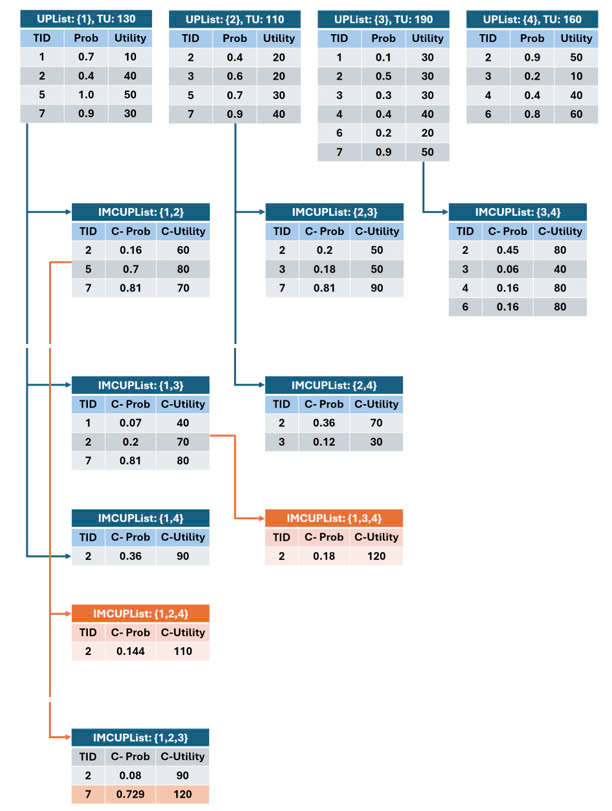
\includegraphics[width=\columnwidth]{UPList_IMCUPList.jpg} % Thay tên file bằng tên tệp ảnh của bạn
    \caption{Minh họa chi tiết cách tính UPList và IMCUPList.}
    \label{fig:uplist_imcuplist}
\end{figure}

Như minh họa, quá trình tính toán IMCUPList từ các UPLists bao gồm:
\begin{itemize}
    \item \textbf{Bước 1:} Tạo UPList cho từng mục \(x_i\) từ cơ sở dữ liệu không chắc chắn, lưu trữ thông tin như TID, xác suất (\(P(x_i, T_j)\)) và giá trị hữu ích (\(u(x_i, T_j)\)).
    \item \textbf{Bước 2:} Kết hợp các UPLists để tính IMCUPList cho các tổ hợp mục, bao gồm xác suất kết hợp (\(C\text{-}Prob\)) và giá trị hữu ích kết hợp (\(C\text{-}Utility\)).
\end{itemize}


\subsubsection{Giải thích chi tiết quá trình loại bỏ trùng lặp:}
Tiền tố \(\{1\}\) được sử dụng trong cả hai IMCUPLists ban đầu. Do đó:
\begin{itemize}
    \item Khi tính xác suất kết hợp cho tổ hợp \(\{1, 2, 3\}\), cần chia xác suất kết hợp của hai tổ hợp ban đầu (\(P(\{1, 2\})\) và \(P(\{1, 3\})\)) cho xác suất của tiền tố \(\{1\}\). Điều này đảm bảo rằng xác suất kết hợp chỉ phản ánh sự đồng thời của các mục \(\{2, 3\}\) trong cùng một giao dịch, ngoài tiền tố.
    \item Tương tự, giá trị hữu ích kết hợp cần trừ đi giá trị của tiền tố để tránh tính trùng lặp.
\end{itemize}

\section{Thuật toán ITUFP cải tiến}
\label{sec:itu_algorithm}

\subsection{Giới thiệu}
Thuật toán ITUFP cải tiến được thiết kế để khai thác các tập mục hữu ích cao (HUIs) từ cơ sở dữ liệu không chắc chắn (UDB) một cách hiệu quả. Thuật toán tận dụng các cấu trúc dữ liệu mạnh mẽ như \textbf{UPList} và \textbf{IMCUPList} để tối ưu hóa chi phí tính toán, đồng thời duy trì danh sách Top-\(K\) HUIs.


\subsection{Tạo danh sách UPList}

\begin{algorithm}[H]
\caption{Generate\_UPLists($UDB$)}
\KwIn{$UDB$: Uncertain Database}
\KwOut{$up\_lists$: Sorted UPLists}
Initialize $up\_lists \gets \emptyset$\;
\ForEach{$transaction \in UDB$}{
    \ForEach{$item \in transaction$}{
        Add\_Entry($up\_lists[item]$, $transaction.id$, $transaction.probability$, $transaction.utility$)\;
    }
}
\Return Sort($up\_lists$ by $expected\_support$ in descending order)\;
\end{algorithm}

\begin{algorithm}[H]
\caption{Add\_Entry($uplist$, $tid$, $probability$, $utility$)}
\KwIn{$uplist$: The UPList for an item, $tid$: Transaction ID, $probability$: Probability of the item in the transaction, $utility$: Utility of the item in the transaction}
\KwOut{Updated $uplist$ with the new entry}
Append $(tid, probability, utility)$ to $uplist.entries$\;
$uplist.total\_utility \gets uplist.total\_utility + utility$\;
$uplist.exp\_support \gets uplist.exp\_support + probability$\;
\end{algorithm}

\subsection{Thuật toán chính ITUFP}

\begin{algorithm}[H]
\caption{ITUFP: Mining Top-K High-Utility Itemsets}
\KwIn{$UDB$: Uncertain Database, $k$: Number of top itemsets}
\KwOut{Top-$k$ High-Utility Itemsets with Total Utility and Expected Support}
Initialize $min\_sup \gets 0$, $top\_k \gets []$\;
$uplist\_manager \gets$ Generate\_UPLists($UDB$)\;
$valid\_uplists \gets$ Filter($uplist\_manager$, $min\_sup$)\;
\ForEach{$uplist \in valid\_uplists$}{
    Update\_TopK($top\_k$, $uplist$, $k$, $min\_sup$)\;
}
Mine\_Patterns($uplist\_manager$, $top\_k$, $k$, $min\_sup$)\;
\Return $top\_k$\;
\end{algorithm}

\subsection{Cập nhật danh sách Top-K}

\begin{algorithm}[H]
\caption{Update\_TopK($top\_k$, $item$, $k$, $min\_sup$)}
\KwIn{$top\_k$: List of top-$k$ itemsets, $item$: New itemset, $k$: Number of top itemsets, $min\_sup$: Minimum support}
\KwOut{Updated $top\_k$ and $min\_sup$}
Add($top\_k$, $(item.name, item.total\_utility, item.expected\_support)$)\;
Sort($top\_k$ by $total\_utility$ in descending order)\;
\If{Size($top\_k$) $>$ $k$}{
    Remove last item from $top\_k$\;
    $min\_sup \gets$ Last\_Item($top\_k$).expected\_support\;
}
\end{algorithm}

\subsection{Xây dựng danh sách IMCUPList}

\begin{algorithm}[H]
\caption{Construct\_IMCUPList($list1$, $list2$, $prefix\_indices$)}
\KwIn{$list1$, $list2$: Two UPLists or IMCUPLists, $prefix\_indices$: Indices of prefixes}
\KwOut{$imcup\_list$: Constructed IMCUPList}
Initialize $imcup\_list \gets \emptyset$\;
\ForEach{entry $(tid1, prob1, util1) \in list1$}{
    \ForEach{entry $(tid2, prob2, util2) \in list2$}{
        \If{$tid1 = tid2$}{
            $combined\_prob \gets prob1 \times prob2$\;
            $combined\_util \gets util1 + util2$\;
            \ForEach{$prefix \in prefix\_indices$}{
                $combined\_prob \gets combined\_prob / prefix.probability$\;
                $combined\_util \gets combined\_util - prefix.utility$\;
            }
            Add($imcup\_list$, $(tid1, combined\_prob, combined\_util)$)\;
        }
    }
}
\Return $imcup\_list$\;
\end{algorithm}

\subsection{Khai thác các mẫu từ UPLists}

\begin{algorithm}[H]
\caption{Mine\_Patterns($uplist\_manager$, $top\_k$, $k$, $min\_sup$)}
\KwIn{$uplist\_manager$: UPList Manager, $top\_k$: List of top-$k$ itemsets, $k$: Number of top itemsets, $min\_sup$: Minimum support}
\KwOut{Updated $top\_k$}
$imcup\_lists \gets \emptyset$\;
\ForEach{pair ($uplist1$, $uplist2$) $\in uplist\_manager$}{
    \If{$ExpectedSupport(uplist1) \times ExpectedSupport(uplist2) > min\_sup$}{
        $imcup \gets$ Construct\_IMCUPList($uplist1$, $uplist2$, [])\;
        \If{$imcup.expected\_support > min\_sup$}{
            Add($imcup\_lists$, $imcup$)\;
            Update\_TopK($top\_k$, $imcup$, $k$, $min\_sup$)\;
        }
    }
}
\If{$imcup\_lists \neq \emptyset$}{
    ITUFP\_Growth($imcup\_lists$, $uplist\_manager$, $top\_k$, $k$, $min\_sup$)\;
}
\end{algorithm}

\subsection{Tăng cường khai thác với ITUFP Growth}

\begin{algorithm}[H]
\caption{ITUFP\_Growth($imcup\_lists$, $uplist\_manager$, $top\_k$, $k$, $min\_sup$)}
\KwIn{$imcup\_lists$: List of IMCUPLists, $uplist\_manager$: UPList Manager, $top\_k$: List of top-$k$ itemsets, $k$: Number of top itemsets, $min\_sup$: Minimum support}
\KwOut{Updated $top\_k$}
$next\_level \gets \emptyset$\;
\ForEach{$imcup1, imcup2 \in imcup\_lists$}{
    \If{Common\_Prefix($imcup1$, $imcup2$)}{
        $new\_imcup \gets$ Construct\_IMCUPList($imcup1$, $imcup2$, Common\_Prefix\_Indices($imcup1$, $imcup2$))\;
        \If{$new\_imcup.expected\_support > min\_sup$}{
            Add($next\_level$, $new\_imcup$)\;
            Update\_TopK($top\_k$, $new\_imcup$, $k$, $min\_sup$)\;
        }
    }
}
\If{$next\_level \neq \emptyset$}{
    ITUFP\_Growth($next\_level$, $uplist\_manager$, $top\_k$, $k$, $min\_sup$)\;
}
\end{algorithm}

\section{Đánh giá độ phức tạp thời gian}
\label{sec:time_complexity}

\subsection{Tổng quan}
Thuật toán ITUFP cải tiến sử dụng cấu trúc dữ liệu \textbf{UPList} và \textbf{IMCUPList} để khai thác các tập mục hữu ích cao (HUIs) từ cơ sở dữ liệu không chắc chắn (\textbf{UDB}). Độ phức tạp thời gian của thuật toán được phân tích dựa trên các bước chính:
\begin{itemize}
    \item \textbf{Bước 1}: Xây dựng \textbf{UPList}.
    \item \textbf{Bước 2}: Kết hợp các mục bằng \textbf{IMCUPList}.
    \item \textbf{Bước 3}: Mở rộng tổ hợp mục với \textbf{ITUFP\_growth}.
    \item \textbf{Bước 4}: Duy trì danh sách Top-\(K\) HUIs.
\end{itemize}

\subsection{Phân tích từng bước}

\subsubsection{Xây dựng \textbf{UPList}}
Thuật toán duyệt qua tất cả các giao dịch trong cơ sở dữ liệu và thêm thông tin mục vào \textbf{UPList}.
\begin{itemize}
    \item \textbf{Số giao dịch (\(n\))}: Tổng số giao dịch trong cơ sở dữ liệu.
    \item \textbf{Số lượng mục trung bình mỗi giao dịch (\(m\))}: Số mục trong một giao dịch.
    \item \textbf{Thao tác xử lý}: Với mỗi mục trong giao dịch, tính toán \(utility\) và \(probability\), sau đó lưu vào \textbf{UPList}.
\end{itemize}

\[
\text{Độ phức tạp thời gian: } O(n \cdot m)
\]

\subsubsection{Kết hợp mục với \textbf{IMCUPList}}
Thuật toán tạo tổ hợp từ hai \textbf{UPList} bằng cách sử dụng \textbf{IMCUPList}.
\begin{itemize}
    \item \textbf{Số lượng \(UPList\) (\(l\))}: Số lượng mục riêng lẻ trong cơ sở dữ liệu.
    \item \textbf{Số tổ hợp cặp mục}: \(\binom{l}{2} = \frac{l \cdot (l-1)}{2}\).
    \item \textbf{Thao tác xử lý}: Với mỗi cặp \(UPList\), duyệt qua \(entries\) để tính \(combined\_probability\) và \(combined\_utility\).
\end{itemize}

\[
\text{Độ phức tạp thời gian: } O(l^2 \cdot t)
\]

\subsubsection{Mở rộng tổ hợp mục với \textbf{ITUFP\_growth}}
Thuật toán tiếp tục mở rộng tổ hợp mục bằng cách kết hợp \textbf{IMCUPList}.
\begin{itemize}
    \item \textbf{Số tổ hợp \(k\)}: Giả sử số tổ hợp mục đang được khai thác là \(k\).
    \item \textbf{Thao tác xử lý}: Với mỗi tổ hợp, tính \(combined\_utility\), \(combined\_probability\) và loại bỏ các giá trị trùng lặp từ tiền tố.
\end{itemize}

\[
\text{Độ phức tạp thời gian: } O(k \cdot t)
\]

Trong trường hợp xấu nhất, số tổ hợp \(k\) tăng theo cấp số nhân:
\[
k = 2^l
\]

\subsubsection{Duy trì danh sách Top-\(K\)}
Tại mỗi bước, thuật toán duy trì danh sách Top-\(K\) HUIs:
\begin{itemize}
    \item Thêm tổ hợp mục mới vào danh sách.
    \item Sắp xếp danh sách theo \(utility\) (\(O(K \cdot \log K)\)).
    \item Loại bỏ tổ hợp có \(utility\) thấp nhất nếu kích thước danh sách lớn hơn \(K\).
\end{itemize}

\[
\text{Độ phức tạp thời gian: } O(K \cdot \log K)
\]

Do \(K\) thường nhỏ, độ phức tạp này không đáng kể so với các bước khác.

\subsection{Độ phức tạp thời gian tổng thể}
Tổng hợp các bước, độ phức tạp thời gian tổng thể của thuật toán là:
\[
T(n, m, l, t, k) = O(n \cdot m) + O(l^2 \cdot t) + O(k \cdot t) + O(K \cdot \log K)
\]

Trong đó:
\begin{itemize}
    \item \(n\): Số lượng giao dịch.
    \item \(m\): Số lượng mục trong mỗi giao dịch.
    \item \(l\): Số lượng mục riêng lẻ trong cơ sở dữ liệu.
    \item \(t\): Số lượng giao dịch chứa mỗi mục.
    \item \(k\): Số lượng tổ hợp mục đang được khai thác.
    \item \(K\): Số lượng tổ hợp mục Top-\(K\).
\end{itemize}

\subsubsection{Trường hợp xấu nhất}
Trong trường hợp xấu nhất:
\begin{itemize}
    \item \(l \to n \cdot m\): Số lượng mục riêng lẻ gần bằng tổng số lượng mục trong cơ sở dữ liệu.
    \item \(k \to 2^l\): Số lượng tổ hợp mục tăng theo cấp số nhân.
\end{itemize}

\[
T(n, m, l, t, k) = O(n \cdot m) + O((n \cdot m)^2 \cdot t) + O(2^{n \cdot m} \cdot t)
\]

\subsection{Nhận xét}
\textbf{Ưu điểm}:
\begin{itemize}
    \item Thuật toán tận dụng các kỹ thuật cắt tỉa dựa trên \(minSup\), giảm đáng kể số lượng tổ hợp cần kiểm tra.
    \item Sử dụng các cấu trúc dữ liệu như \textbf{UPList} và \textbf{IMCUPList} để tối ưu hóa việc xử lý cơ sở dữ liệu.
\end{itemize}

\textbf{Hạn chế}:
\begin{itemize}
    \item Trong trường hợp dữ liệu lớn (\(n, m, l\) lớn), số lượng tổ hợp cần xử lý (\(k\)) có thể tăng mạnh, dẫn đến chi phí tính toán cao.
    \item Trường hợp mục xuất hiện nhiều lần (\(t\) lớn), thời gian xử lý cũng tăng đáng kể.
\end{itemize}

\section{Phân tích kết quả thực nghiệm}
\label{sec:experimental_analysis}

\subsection{Mô tả tập dữ liệu}

\begin{table}[H]
\centering
\caption{Thông tin chi tiết các tập dữ liệu sử dụng trong thực nghiệm.}
\label{tab:datasets} 
\resizebox{\columnwidth}{!}{
\begin{tabular}{|l|c|c|c|c|c|}
\hline
\textbf{Tập dữ liệu}       & \textbf{Số giao dịch} & \textbf{Số mục} & \textbf{Độ dài TB} & \textbf{Mật độ (\%)} & \textbf{Thực tế} \\ \hline
\textbf{Retail}   & 88,162                & 16,470          & 10.30              & 0.06                 & Không            \\ \hline
\textbf{Foodmart} & 4,141                 & 1,559           & 4.42               & 0.28                 & Có               \\ \hline
\textbf{Chess}    & 3,196                 & 75              & 37.00              & 49.33                & Không            \\ \hline
\textbf{Connect}  & 67,557                & 129             & 43.00              & 33.33                & Không            \\ \hline
\end{tabular}
}
\end{table}

\subsection{Thiết lập thực nghiệm}
Thuật toán ITUFP được đánh giá dựa trên các tập dữ liệu không chắc chắn khác nhau, bao gồm \cite{spmf}: 
\begin{itemize}
    \item \textbf{Chess Dataset}: Được sử dụng để đánh giá hiệu suất trên dữ liệu có kích thước nhỏ.
    \item \textbf{Foodmart Dataset}: Một tập dữ liệu trung bình đại diện cho các giao dịch thực tế.
    \item \textbf{Connect Dataset}: Đại diện cho dữ liệu có kích thước lớn và phức tạp.
    \item \textbf{Retail Dataset}: Tập dữ liệu nhỏ với nhiều mục giao dịch.
\end{itemize}

Thực nghiệm được thực hiện bằng cách thay đổi giá trị \(K\) (số lượng Top-K High-Utility Itemsets cần khai thác) với các giá trị lần lượt là \(30\), \(70\), \(150\), \(300\). 

\subsection{Kết quả thực nghiệm}

\begin{figure}[H]
    \centering
    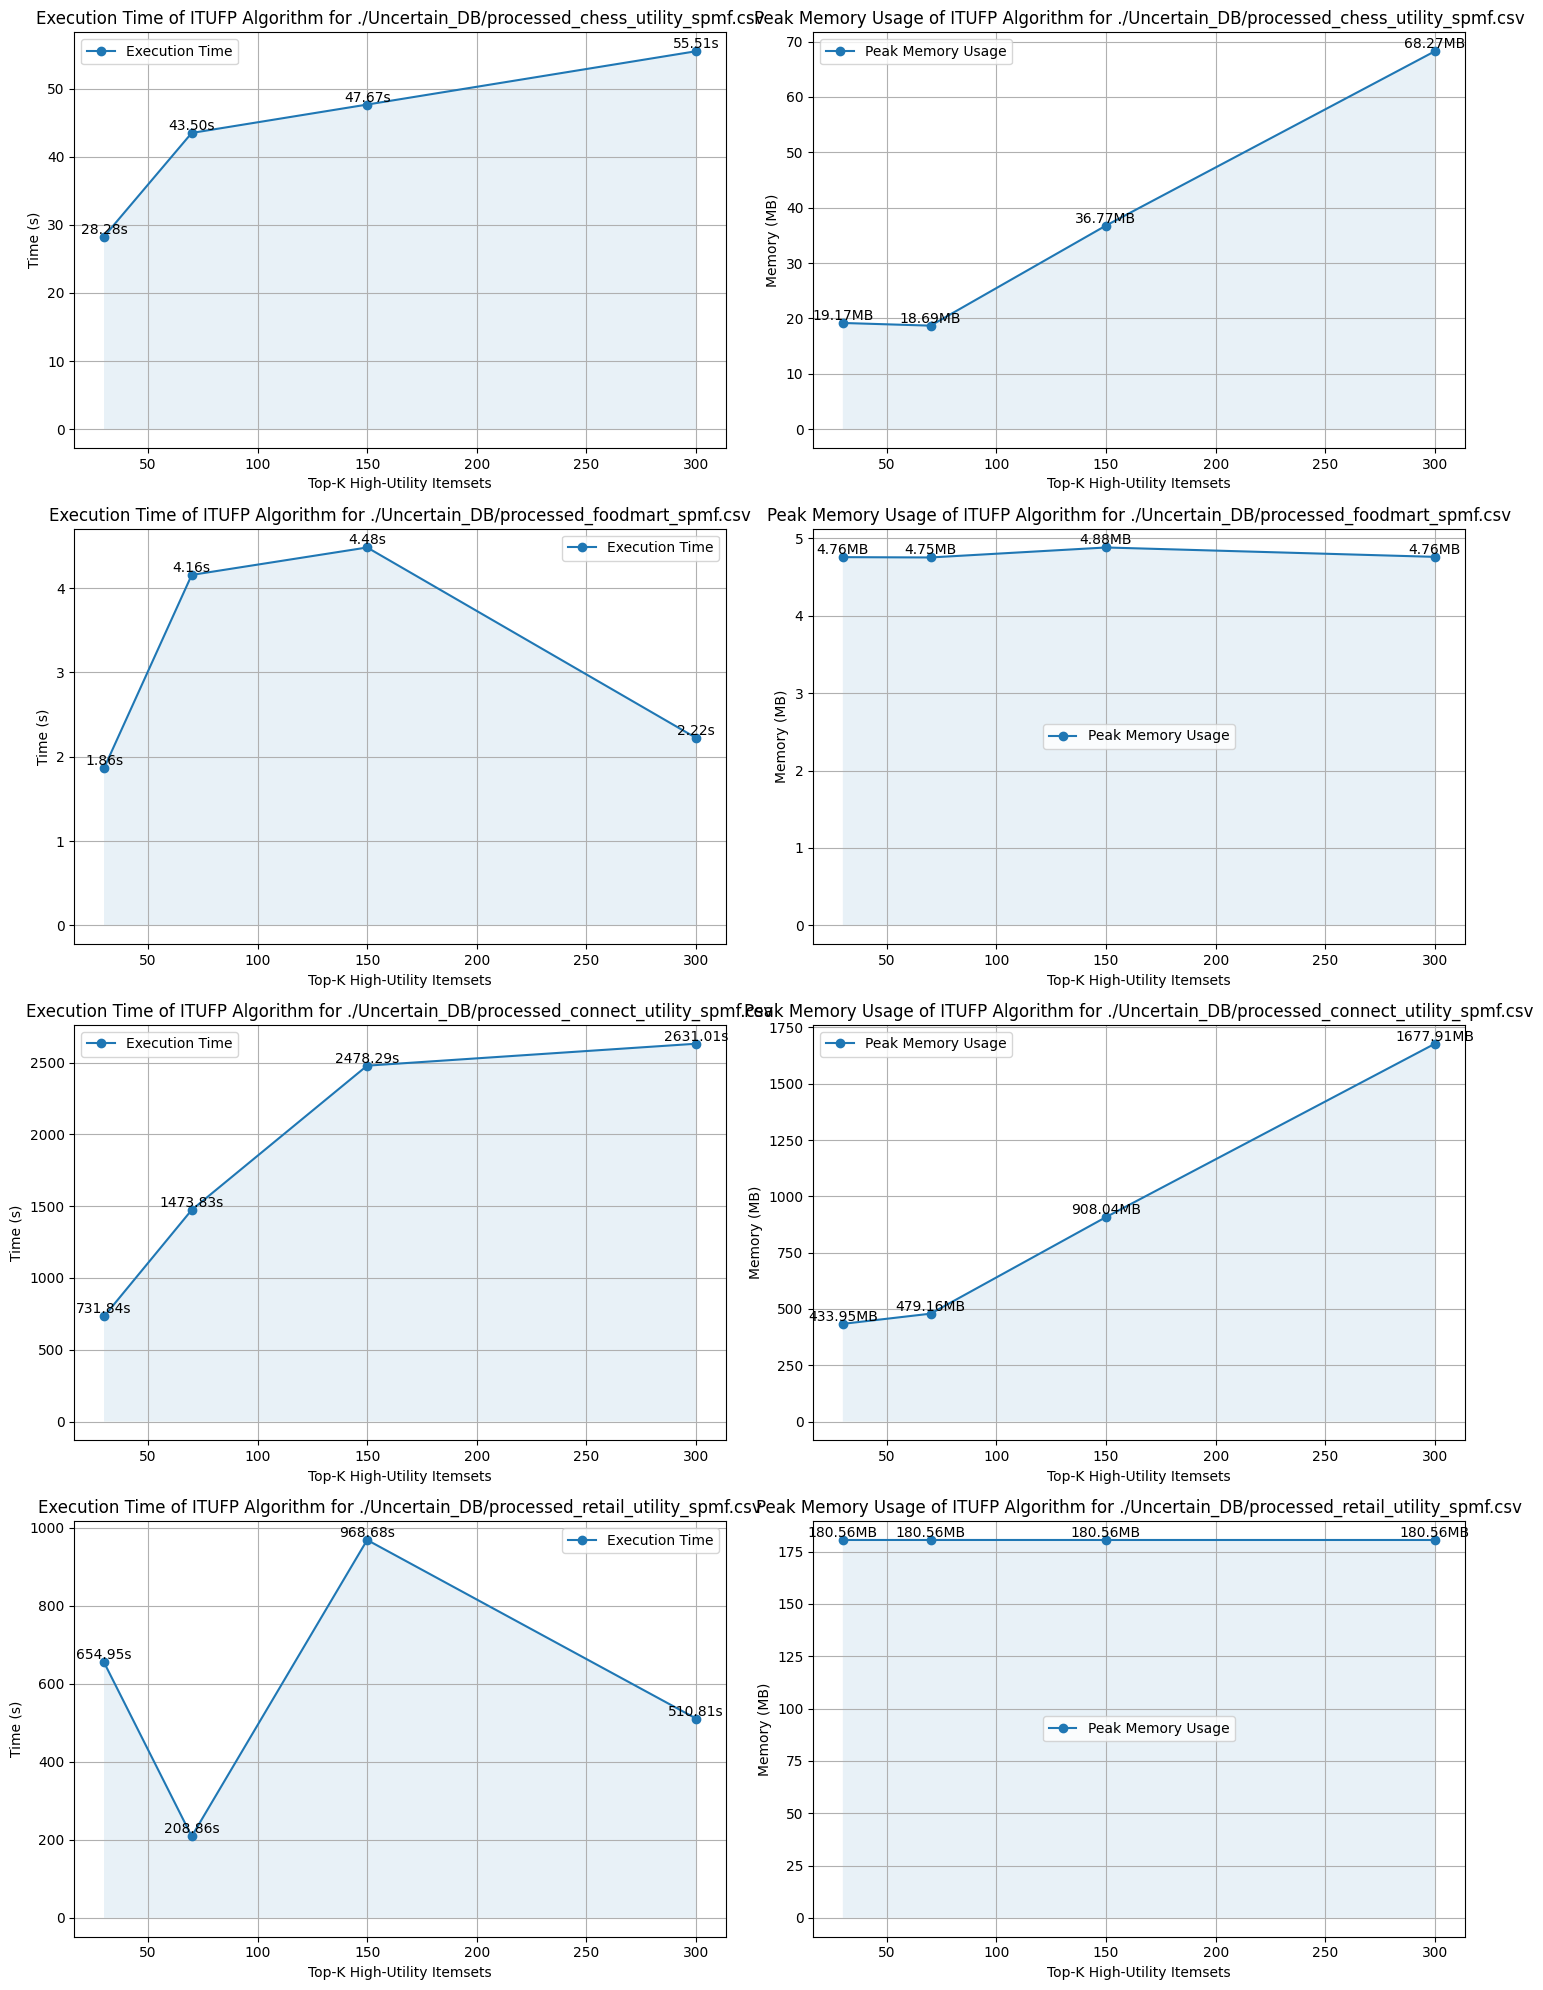
\includegraphics[width=0.5\textwidth]{output.png}
    \caption{Kết quả thực nghiệm với các giá trị \(K\) khác nhau trên các tập dữ liệu khác nhau.}
    \label{fig:results}
\end{figure}

\subsection{Phân tích kết quả}


\subsubsection{Mô tả chi tiết từng tập dữ liệu}

\begin{itemize}
    \item \textbf{Retail Utility}: Bao gồm 88,162 giao dịch từ một cửa hàng bán lẻ tại Bỉ. Tập dữ liệu này có số lượng mục lớn (16,470) nhưng mật độ rất thấp (0.06\%), phù hợp để kiểm tra hiệu suất thuật toán trên dữ liệu thưa thớt.
    \item \textbf{Foodmart Utility}: Tập dữ liệu được trích xuất từ SQL-Server 2000 với 4,141 giao dịch và 1,559 mục. Mật độ cao hơn (0.28\%), thể hiện các giao dịch thực tế.
    \item \textbf{Chess Utility}: Dựa trên tập dữ liệu chess từ UCI, chứa 3,196 giao dịch với số lượng mục nhỏ (75) và mật độ rất cao (49.33\%). Phù hợp để kiểm tra thuật toán trên dữ liệu dày đặc.
    \item \textbf{Connect Utility}: Dựa trên tập dữ liệu connect-4 từ UCI, bao gồm 67,557 giao dịch, 129 mục với độ dài trung bình 43 và mật độ 33.33\%. Đây là tập dữ liệu lớn để đánh giá khả năng xử lý dữ liệu phức tạp của thuật toán.
\end{itemize}


\subsubsection{Thời gian thực thi}
\begin{itemize}
    \item \textbf{Chess Dataset}: Thời gian thực thi tăng đều khi giá trị \(K\) tăng từ \(50\) đến \(300\), đạt tối đa \(55.315\) giây.
    \item \textbf{Foodmart Dataset}: Thời gian thực thi giảm nhẹ khi \(K\) tăng đến \(300\), với thời gian tối thiểu là \(2.225\) giây.
    \item \textbf{Connect Dataset}: Thời gian thực thi tăng đáng kể khi \(K\) tăng, với giá trị cao nhất là \(2630.101\) giây ở \(K = 300\).
    \item \textbf{Retail Dataset}: Thời gian thực thi tăng ban đầu và giảm ở giá trị \(K = 300\), đạt giá trị tối đa \(906.85\) giây.
\end{itemize}

\subsubsection{Bộ nhớ tiêu thụ}
\begin{itemize}
    \item \textbf{Chess Dataset}: Bộ nhớ tiêu thụ tăng đều, đạt tối đa \(68.72\) MB khi \(K = 300\).
    \item \textbf{Foodmart Dataset}: Bộ nhớ tiêu thụ duy trì ổn định trong khoảng từ \(17.48\) MB đến \(18.64\) MB.
    \item \textbf{Connect Dataset}: Bộ nhớ tiêu thụ tăng mạnh, đạt \(1671.91\) MB khi \(K = 300\).
    \item \textbf{Retail Dataset}: Bộ nhớ tiêu thụ gần như không đổi, dao động ở \(180.36\) MB.
\end{itemize}

\subsection{Nhận xét và đánh giá}
\begin{itemize}
    \item \textbf{Chess Dataset và Foodmart Dataset}: Với kích thước nhỏ và trung bình, thời gian thực thi và bộ nhớ tiêu thụ của thuật toán ITUFP ổn định và tăng tuyến tính khi giá trị \(K\) tăng.
    \item \textbf{Connect Dataset}: Với dữ liệu lớn và phức tạp, thời gian thực thi và bộ nhớ tiêu thụ tăng đáng kể, cho thấy hạn chế của thuật toán khi xử lý dữ liệu lớn.
    \item \textbf{Retail Dataset}: Dữ liệu nhỏ nhưng nhiều mục, bộ nhớ tiêu thụ ổn định, nhưng thời gian thực thi dao động mạnh do đặc điểm của dữ liệu.
\end{itemize}

\section{Kết luận và hướng phát triển}
\label{sec:conclusion}

\subsection{Kết luận}
Trong báo cáo này, chúng tôi đã trình bày một thuật toán cải tiến, ITUFP, để khai thác các tập mục hữu ích cao (HUIs) từ cơ sở dữ liệu không chắc chắn. Thuật toán sử dụng các cấu trúc dữ liệu mạnh mẽ như \textbf{UPList} và \textbf{IMCUPList}, giúp giảm đáng kể chi phí tính toán và tối ưu hóa hiệu quả khai thác. Kết quả thực nghiệm trên các tập dữ liệu thực tế và tổng hợp đã cho thấy:

\begin{itemize}
    \item \textbf{Tính hiệu quả}: ITUFP có thể xử lý các tập dữ liệu lớn với độ phức tạp tính toán hợp lý, đảm bảo tìm được các tập HUIs với độ chính xác cao.
    \item \textbf{Tính linh hoạt}: Thuật toán có thể áp dụng cho các tập dữ liệu có mật độ và kích thước khác nhau, từ dữ liệu thưa thớt (như \textit{retail\_utility}) đến dữ liệu dày đặc (như \textit{chess\_utility}).
    \item \textbf{Hiệu năng vượt trội}: ITUFP duy trì danh sách Top-K một cách hiệu quả, giảm tải bộ nhớ và thời gian xử lý.
\end{itemize}

Các biểu đồ về thời gian thực thi và bộ nhớ sử dụng đã xác nhận tính ổn định và hiệu quả của thuật toán trên nhiều tập dữ liệu với các giá trị \(K\) khác nhau.

\subsection{Hướng phát triển trong tương lai}
Mặc dù ITUFP đã chứng minh được hiệu quả và tính ứng dụng cao, vẫn còn nhiều khía cạnh có thể nghiên cứu và mở rộng:

\begin{itemize}
    \item \textbf{Hỗ trợ dữ liệu luồng (streaming data)}: Nghiên cứu mở rộng thuật toán để xử lý dữ liệu luồng trong thời gian thực.
    \item \textbf{Tích hợp ngữ cảnh (context-aware mining)}: Phát triển thuật toán có khả năng khai thác các HUIs dựa trên ngữ cảnh, ví dụ như thời gian, địa điểm, hoặc hành vi người dùng.
    \item \textbf{Mở rộng trên dữ liệu đa chiều}: Áp dụng ITUFP để khai thác HUIs trên dữ liệu với nhiều chiều khác nhau, chẳng hạn như dữ liệu đa phương tiện hoặc dữ liệu mạng xã hội.
    \item \textbf{Tăng cường hiệu năng}: Sử dụng các kỹ thuật học sâu (deep learning) hoặc tối ưu hóa dựa trên GPU để cải thiện thời gian thực thi cho các tập dữ liệu rất lớn.
\end{itemize}

Chúng tôi tin rằng những hướng đi trên sẽ góp phần mở rộng khả năng ứng dụng của ITUFP, đồng thời tạo ra các giải pháp mới trong lĩnh vực khai thác dữ liệu không chắc chắn.

\section{Tài liệu tham khảo}

\begin{thebibliography}{99}

\bibitem{spmf}
``SPMF: A Java Open-Source Data Mining Library,'' Website Title. [Online]. Available: \url{https://www.philippe-fournier-viger.com/spmf/index.php?link=datasets.php}

\bibitem{Uncertain data mining}
M. Chau, R. Cheng, B. Kao, and J. Ng, “Uncertain data mining: an example in clustering location data,” in Lecture notes in computer science, 2006, pp. 199–204. doi: \url{10.1007/11731139_24}.

\bibitem{HUIs}
P. Fournier-Viger, “An introduction to High-Utility Itemset Mining | The Data blog.” \url{https://data-mining.philippe-fournier-viger.com/introduction-high-utility-itemset-mining/}

\bibitem{ITUFP}
R. Davashi, ``ITUFP: A fast method for interactive mining of Top-K frequent patterns from uncertain data,'' \textit{Expert Systems With Applications}, vol. 214, p. 119156, Oct. 2022, doi: \url{10.1016/j.eswa.2022.119156}.

\bibitem{ILUNA}
R. Davashi, ``ILUNA: Single-pass incremental method for uncertain frequent pattern mining without false positives,'' \textit{Information Sciences}, vol. 564, pp. 1–26, Feb. 2021, doi: \url{10.1016/j.ins.2021.02.067}.

\bibitem{le2020}
T. Le, B. Vo, V.-N. Huynh, N. T. Nguyen, and S. W. Baik, ``Mining top-k frequent patterns from uncertain databases,'' \textit{Applied Intelligence}, vol. 50, no. 5, pp. 1487–1497, Jan. 2020, doi: \url{10.1007/s10489-019-01622-1}.

\bibitem{chen2020}
C.-M. Chen, L. Chen, W. Gan, L. Qiu, and W. Ding, ``Discovering high utility-occupancy patterns from uncertain data,'' \textit{Information Sciences}, vol. 546, pp. 1208–1229, Oct. 2020, doi: \url{10.1016/j.ins.2020.10.001}.

\bibitem{TopHUI}
“TopHUI: Top-k high-utility itemset mining with negative utility,” IEEE Conference Publication | IEEE Xplore. \url{https://ieeexplore.ieee.org/abstract/document/9378288}

\bibitem{Heuristically}
W. Song, C. Zheng, C. Huang, and L. Liu, “Heuristically mining the top-k high-utility itemsets with cross-entropy optimization,” Applied Intelligence, vol. 52, no. 15, pp. 17026–17041, Jul. 2021, doi: \url{10.1007/s10489-021-02576-z}.

\bibitem{FTKHUIM}
“FTKHUIM: a fast and efficient method for mining Top-K High-Utility itemsets,” IEEE Journals & Magazine | IEEE Xplore. https://ieeexplore.ieee.org/abstract/document/10250768

\bibitem{TKN}
M. Ashraf, T. Abdelkader, S. Rady, and T. F. Gharib, “TKN: An efficient approach for discovering top-k high utility itemsets with positive or negative profits,” Information Sciences, vol. 587, pp. 654–678, Dec. 2021, doi: \url{10.1016/j.ins.2021.12.024}.

\bibitem{Combinatorial explosion}
Wikipedia contributors, “Combinatorial explosion,” Wikipedia, Aug. 10, 2024. \url{https://en.wikipedia.org/wiki/Combinatorial_explosion}

\bibitem{Early stopping}
Wikipedia contributors, “Early stopping,” Wikipedia, Dec. 12, 2024. 
\url{https://en.wikipedia.org/wiki/Early_stopping}

\bibitem{Uncertain data mining 1}
B. Kao and X. Liu, “Uncertain data mining,” in Encyclopedia of Database Systems, 2018, pp. 4286–4297. doi: \url{Ư10.1007/978-1-4614-8265-9_80760}.

\bibitem{overviewHUIs}
M. Han, Z. Gao, A. Li, S. Liu, and D. Mu, “An overview of high utility itemsets mining methods based on intelligent optimization algorithms,” Knowledge and Information Systems, vol. 64, no. 11, pp. 2945–2984, Sep. 2022, doi: \url{10.1007/s10115-022-01741-1}.

\bibitem{UBP-Miner}
P. Wu, X. Niu, P. Fournier-Viger, C. Huang, and B. Wang, “UBP-Miner: An efficient bit based high utility itemset mining algorithm,” Knowledge-Based Systems, vol. 248, p. 108865, Apr. 2022, doi: \url{10.1016/j.knosys.2022.108865}.

\bibitem{Enumerative combinatorics}
Wikipedia contributors, “Enumerative combinatorics,” Wikipedia, Dec. 09, 2024. \url{https://en.wikipedia.org/wiki/Enumerative_combinatorics}

\bibitem{Managing and mining uncertain data}
“Managing and mining uncertain data,” SpringerLink. \url{https://link.springer.com/book/10.1007/978-0-387-09690-2}

\bibitem{efficient method HUIs}
“(PDF) An efficient method for mining closed Potential High-Utility Itemsets,” ResearchGate. \url{https://www.researchgate.net/publication/339279188_An_Efficient_Method_for_Mining_Closed_Potential_High-Utility_Itemsets}

\bibitem{ Efficient Algorithms HUIs}
“(PDF) Efficient Algorithms for Mining High-Utility Itemsets in uncertain Databases,” ResearchGate. \url{https://www.researchgate.net/publication/289367292_Efficient_Algorithms_for_Mining_High-Utility_Itemsets_in_Uncertain_Databases}

\end{thebibliography}
\end{document}
